\documentclass[a4paper,12]{article}

%\usepackage{times}
\usepackage{fancyhdr}
\usepackage[utf8]{inputenc}
\usepackage{circuitikz}
\usepackage[top=2cm,bottom=2cm,right=2cm,left=2cm]{geometry}
\usepackage{array}
\usepackage{multirow}
\usepackage{hhline}
\usepackage{float}
\usepackage{karnaugh-map}
\usepackage{lastpage}

\newcommand{\olsi}[1]{\,\overline{\!{#1}}} % overline short italic
\newcommand{\ols}[1]{\mskip.5\thinmuskip\overline{\mskip-.5\thinmuskip {#1} \mskip-.5\thinmuskip}\mskip.5\thinmuskip} % overline short

\pagestyle{fancy}   
\lhead{Applied Digital Electronics}
\rhead{Group Assignment 2}
\cfoot{Page \thepage of \pageref{LastPage}}


\begin{document}

\begin{figure}[H]
    \centering
    
\includegraphics{mak_logo.png}
\end{figure}
\begin{center}
\textbf {COLLEGE OF ENGINEERING, DESIGN, ART AND TECHNOLOGY\\[10pt]
DEPARTMENT OF ELECTRICAL AND COMPUTER ENGINEERING\\[10pt]
SCHOOL OF ENGINEERING\\[10pt]
BACHELOR OF SCIENCE IN ELECTRICAL ENGINEERING\\[10pt]
YEAR THREE\\[10pt]
ELE3103: APPLIED DIGITAL ELECTRONICS\\[10pt]
GROUP ASSIGNMENT 2\\[20pt]
GROUP MEMBERS\\
}\end{center}
\begin{center}
    \begin{tabular}{|l|c|c|c|}
        \hline
    \textbf{NAME} & \textbf{COURSE} & \textbf{REG. NO.}\\[10pt] \hline
    Babirye Immaculate & BELE & 21/U/1048 \\[10pt] \hline
    Akirapa Jacky & BELE & 21/U/0637 \\[10pt] \hline
    Nabwire Jovia Namulinda & BELE & 21/U/1352 \\[10pt] \hline
    Mbalire Shawal & BELE & 21/U/0851 \\[10pt] \hline
    Bwire Kennedy & BELE & 21/U/0456 \\[10pt] \hline
    \end{tabular} \\[20pt]
    \textbf{\date{\today}}\\[10pt]
    \textbf{SUPERVISOR: Dr EDWIN MUGUME}
\end{center}




\newpage
\section*{Question One}
The following figure shows the intersection of a main highway with a secondary
access road. Vehicle-detection sensors are placed along lanes C and D (main
road) and lanes A and B (access road). These sensor outputs are LOW (0) when
no vehicle is present and HIGH (1) when a vehicle is present. The intersection
traffic light is to be controlled according to the following logic: 

\begin{enumerate}
\item The East-West (E-W) traffic light is green when both lanes C and D are occupied.
\item The E-W light is green when either C or D is occupied but lanes A and B are both not occupied.
\item The North-South (N-S) light is green whenever both lanes A and B are occupied but C and D are not both occupied.
\item The N-S light is also green when either A or B is occupied while C and D are both vacant.
\item The E-W light is green when no vehicles are present.
There should be two outputs, N-S and E-W, that go HIGH when the corresponding light is to be green.
\end{enumerate}

\begin{figure}[H]
    \centering
    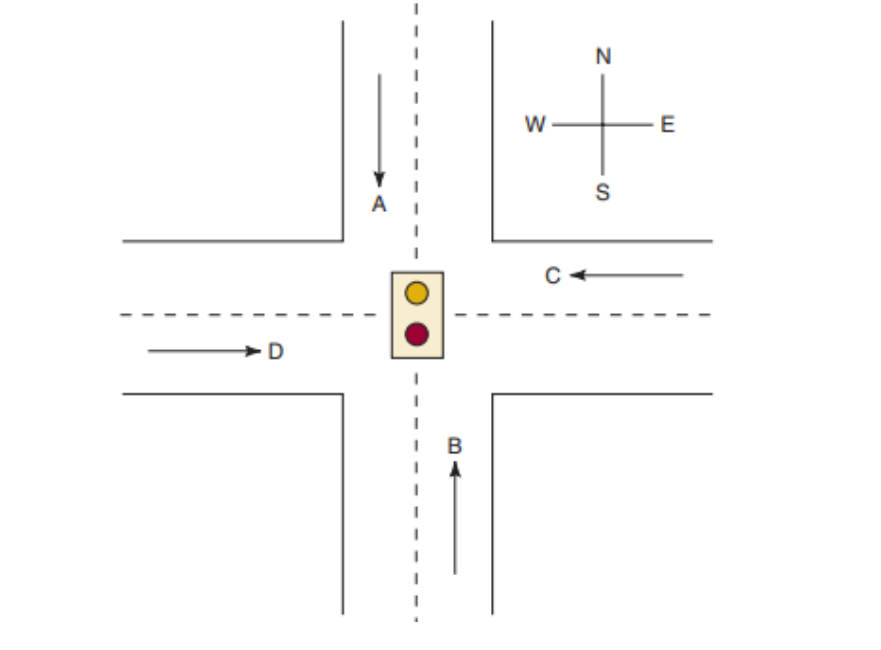
\includegraphics[width=0.6\linewidth]{q1.png}
    \caption{The intersection of a main highway with a secondary access road}
    \label{fig:q1}
\end{figure}

\subsection*{(a)} \textbf{ Using the sensor outputs A, B, C, and D as inputs, design a logic circuit to
control the traffic light.}

truth table for the logic \\
\begin{center}
\begin{tabular}{cccc|c|c|c}
    A & B & C & D & E-W & N-S &\\ 
    \hline
    0 & 0 & 0 & 0 & 1 & 0 & $\olsi{A}\olsi{B}\olsi{C}\olsi{D}$\\ 
    0 & 0 & 0 & 1 & 1 & 0 & $\olsi{A}\olsi{B}\olsi{C}D$\\ 
    0 & 0 & 1 & 0 & 1 & 0 & $\olsi{A}\olsi{B}C\olsi{D}$\\ 
    0 & 0 & 1 & 1 & 1 & 0 & $\olsi{A}\olsi{B}CD$\\ 
    0 & 1 & 0 & 0 & 0 & 1 & $\olsi{A}B\olsi{C}\olsi{D}$\\ 
    0 & 1 & 0 & 1 & 0 & 0 &\\ 
    0 & 1 & 1 & 0 & 0 & 0 &\\ 
    0 & 1 & 1 & 1 & 1 & 0 & $\olsi{A}BCD$\\ 
    1 & 0 & 0 & 0 & 0 & 1 & $A\olsi{B}\olsi{C}\olsi{D}$\\ 
    1 & 0 & 0 & 1 & 0 & 0 &\\ 
    1 & 0 & 1 & 0 & 0 & 0 &\\ 
    1 & 0 & 1 & 1 & 1 & 0 & $A\olsi{B}CD$\\ 
    1 & 1 & 0 & 0 & 0 & 1 & $AB\olsi{C}\olsi{D}$\\ 
    1 & 1 & 0 & 1 & 0 & 1 & $AB\olsi{C}D$\\ 
    1 & 1 & 1 & 0 & 0 & 1 & $ABC\olsi{D}$\\ 
    1 & 1 & 1 & 1 & 1 & 0 & $ABCD$\\ 
\end{tabular}
\end{center}


\begin{center}
\begin{karnaugh-map}[4][4][1][D][C][B][A]
    \manualterms{1,1,1,1,0,0,0,1,0,0,0,1,0,0,0,1}
    \implicant{3}{11} 
    \implicant{0}{2}
\end{karnaugh-map}
\end{center}
\[ E-W = \olsi{A} \olsi{B} + CD\]

\begin{center}
\begin{karnaugh-map}[4][4][1][D][C][B][A]
    \manualterms{0,0,0,0,1,0,0,0,1,0,0,0,1,1,1,0}
    \implicant{4}{12} 
    \implicant{12}{8}
    \implicant{12}{13}
    \implicantedge{12}{12}{14}{14}
\end{karnaugh-map}
\end{center}
\[N-S = B\olsi{C}\olsi{D}+AB\olsi{C}+A\olsi{C}\olsi{D}+AB\olsi{D}\]

\begin{center}
\begin{circuitikz}

    
    \draw
    (8,10) node[and port] (ABew) {}
    (8, 0) node[and port] (CDew) {}

    (2,11) node[not port, scale = 0.5] (notA) {}
    (3, 9) node[not port, scale = 0.5] (notB) {}
    (4, 7) node[not port, scale = 0.5] (notC) {}
    (5, 5) node[not port, scale = 0.5] (notD) {}

    
    (1, 9) node[] (A) {}
    (2, 7) node[] (B) {}
    (3, 5) node[] (C) {}
    (4, 3) node[] (D) {}

    (0, 9) node[label=left:A] {} to[short,*-*] (A)
    (0, 7) node[label=left:B] {} to[short,*-*] (B)
    (0, 5) node[label=left:C] {} to[short,*-*] (C)
    (0, 3) node[label=left:D] {} to[short,*-*] (D)


    (10,8) node[and port, number inputs=3] (andabc) {}
    (10,6) node[and port, number inputs=3] (andbcd) {}
    (10,4) node[and port, number inputs=3] (andacd) {}
    (10,2) node[and port, number inputs=3] (andabd) {}

    
    (14,10) node[or port, number inputs=2] (orew) {}
    (14,4) node[or port, number inputs=4] (orns) {}

    (notA.out) |- (ABew.in 1)
    (notB.out) |- (ABew.in 2)

    (C) |- (CDew.in 1)
    (D) |- (CDew.in 2)

    (ABew.out) |- (orew.in 1)
    (CDew.out) |- (orew.in 2)

    
    (A)    |- (notA.in 1)
    (B)    |- (notB.in 1)
    (C)    |- (notC.in 1)
    (D)    |- (notD.in 1)

    (A)    |- (andabc.in 1)
    (B)    |- (andabc.in 2)
    (notC.out) |- (andabc.in 3)

    (B)    |- (andbcd.in 1)
    (notC.out) |- (andbcd.in 2)
    (notD.out) |- (andbcd.in 3)

    (A)    |- (andacd.in 1)
    (notC.out) |- (andacd.in 2)
    (notD.out) |- (andacd.in 3)

    (A)    |- (andabd.in 1)
    (B)    |- (andabd.in 2)
    (notD.out) |- (andabd.in 3)

    (andabc.out) |- (orns.in 1)
    (andbcd.out) |- (orns.in 2)
    (andacd.out) |- (orns.in 3)
    (andabd.out) |- (orns.in 4)

    (orns.out) to[short, -o] ++(1,0) node[label=right:$NS$] {}
    (orew.out) to[short, -o] ++(1,0) node[label=right:$EW$] {}
    
    
;\end{circuitikz}
\end{center}

\section*{(b)} \textbf{ Use Quartus software to implement the circuit in (a). Show the code, RTL
viewer schematic, and timing diagram of the circuit performance.}

\begin{figure}[H]
    \centering
    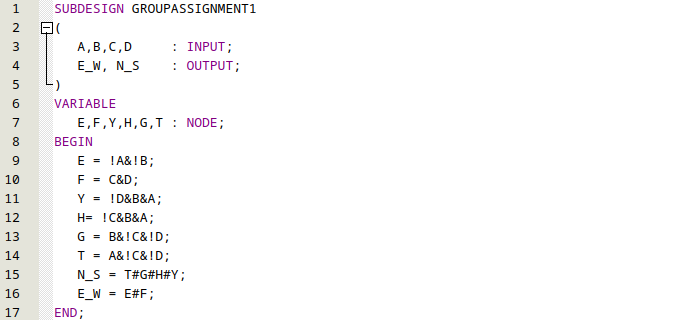
\includegraphics[width=\linewidth]{q1code.png}
    \caption{The AHDL code for the circuit in question 1}
    \label{fig:q1code}  
\end{figure}
\begin{figure}[H]
    \centering
    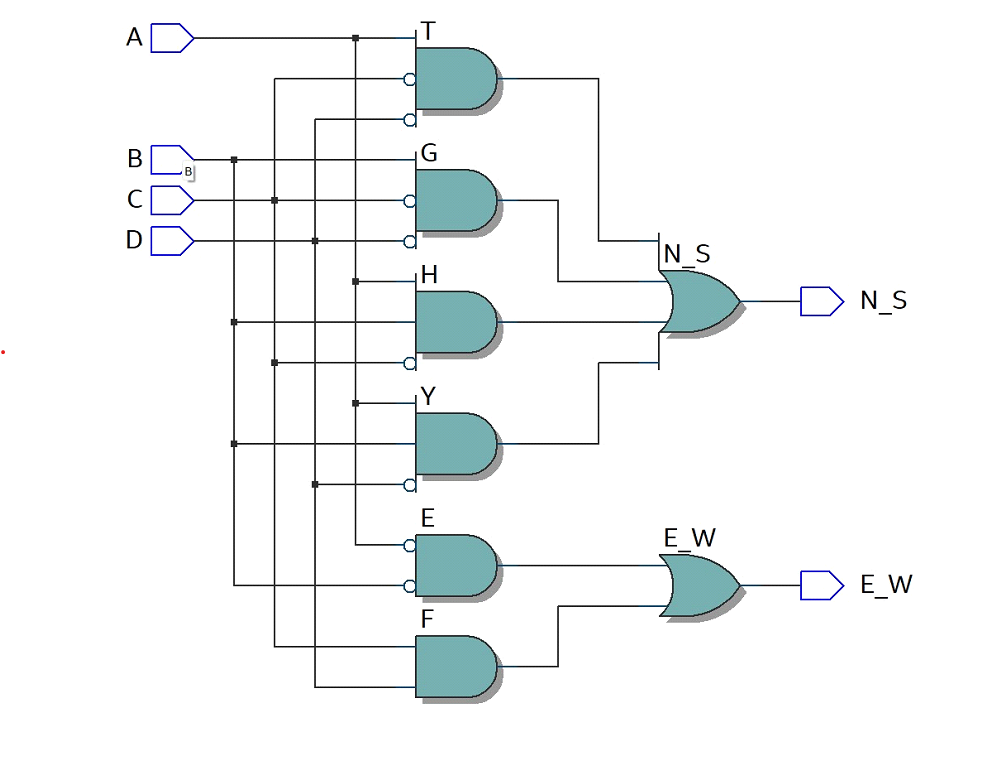
\includegraphics[width=\linewidth]{q1schem.png}
    \caption{The Quartus generated schematic for the circuit in question 1}
    \label{fig:q1schem}    
\end{figure}
\begin{figure}[H]
    \centering
    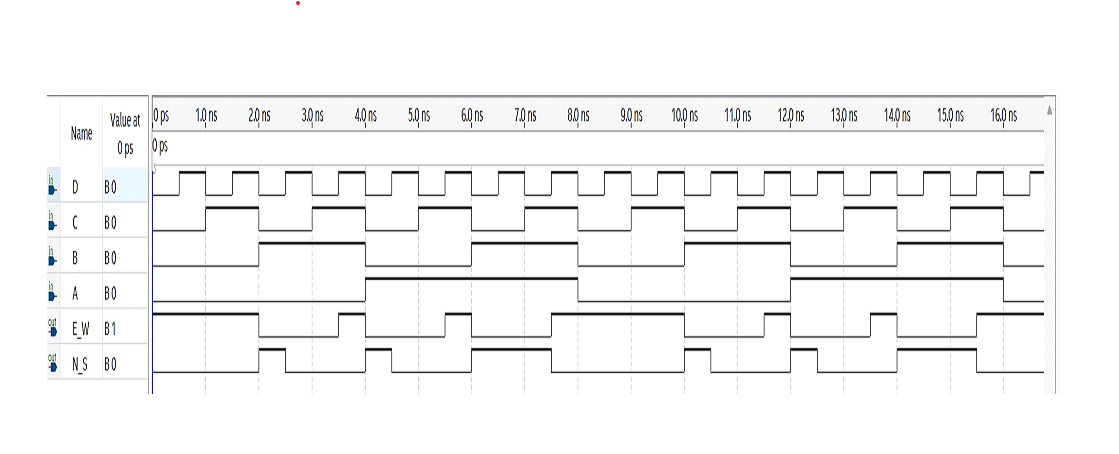
\includegraphics[width=\linewidth]{q1tim.png}
    \caption{Timing diagram for the circuit in question 1}
    \label{fig:q1timi}    
\end{figure}



\newpage
\section*{Question 2}
The following figure shows an automobile alarm circuit used to detect certain
undesirable conditions. The three switches are used to indicate the status of the
door by the driver`s seat, the ignition, and the headlights, respectively.

\begin{figure}[H]
    \centering
    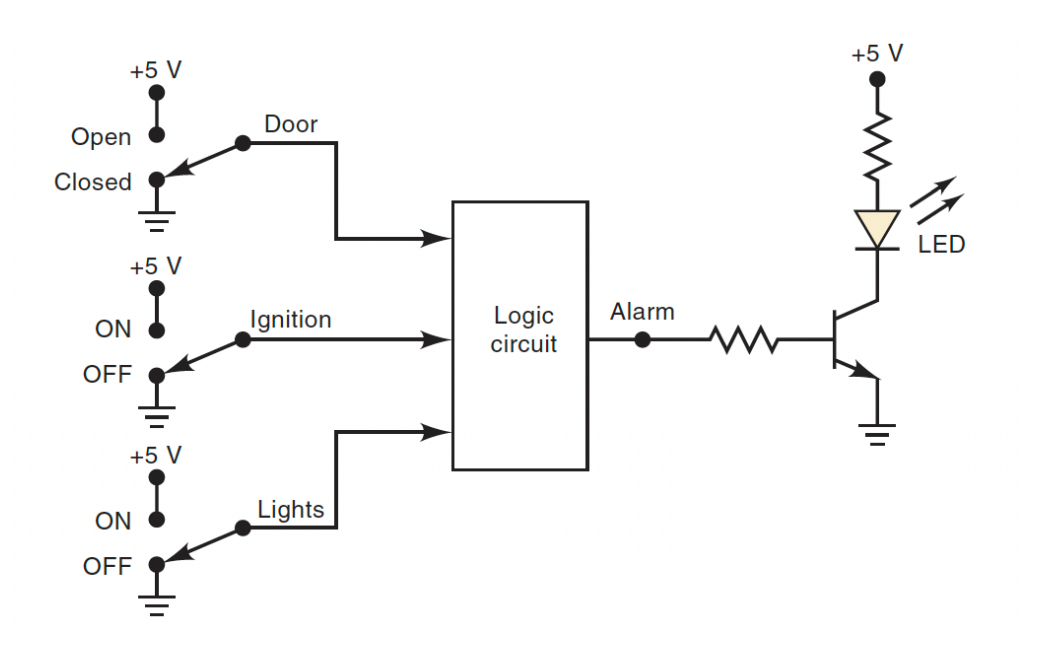
\includegraphics[width=0.6\linewidth]{q2.png}
    \caption{An automobile alarm circuit used to detect certain undesirable conditions}
    \label{fig:q2}
\end{figure}


\subsection*{(a)} \textbf{Design the logic circuit with these three switches as inputs so that the alarm
is activated whenever either of the following conditions exists:
i. The headlights are on while the ignition is off.
ii. The door is open while the ignition is on}

let D = door I = ignition H= lights A = alarm
\begin{center}
\begin{tabular}{ccc|cc}
    H & I & D & A \\ \hline
    0 & 0 & 0 & 0 & \\
    0 & 0 & 1 & 0 &\\
    0 & 1 & 0 & 0 &\\
    0 & 1 & 1 & 1 & $\olsi{H}ID$\\
    1 & 0 & 0 & 1 & $H\olsi{I}\olsi{D}$\\
    1 & 0 & 1 & 1 & $H\olsi{I}D$\\
    1 & 1 & 0 & 0 &\\
    1 & 1 & 1 & 1 & $HID$\\

\end{tabular}
\end{center}
\begin{center}
\begin{karnaugh-map}[4][2][1][D][I][H]
    \manualterms{0,0,0,1,1,1,0,1}
    \implicant{3}{7}
    \implicant{4}{5}
\end{karnaugh-map}
\end{center}

\[A = H\olsi{I} + ID\]

\begin{center}
\begin{circuitikz}
    \draw
    (5,0) node[and port] (IH) {}
    (2,2) node[not port] (notI) {}
    (4,4) node[and port] (ID) {}
    (7,2) node[or port] (or) {}

    (0, 4) node[label=left:D] {} |- (ID.in 1)
    (0, 2) node[label=left:I] {} |- (1, 2)
    (1, 2) |- (notI.in)
    (1, 2) |- (ID.in 2)
    (0, 0) node[label=left:H] {} |- (IH.in 2)

    (notI.out) |- (IH.in 1)

    (IH.out) |- (or.in 2)
    (ID.out) |- (or.in 1)
    (or.out) to[short, -o] ++(1,0) node[label=right:$A$] {};
\end{circuitikz}
\end{center}

\subsection*{(b)} \textbf{Use Quartus software to implement the circuit in (a). Show the code, RTL
viewer schematic, and timing diagram of the circuit performance.}

\begin{figure}[H]
    \centering
    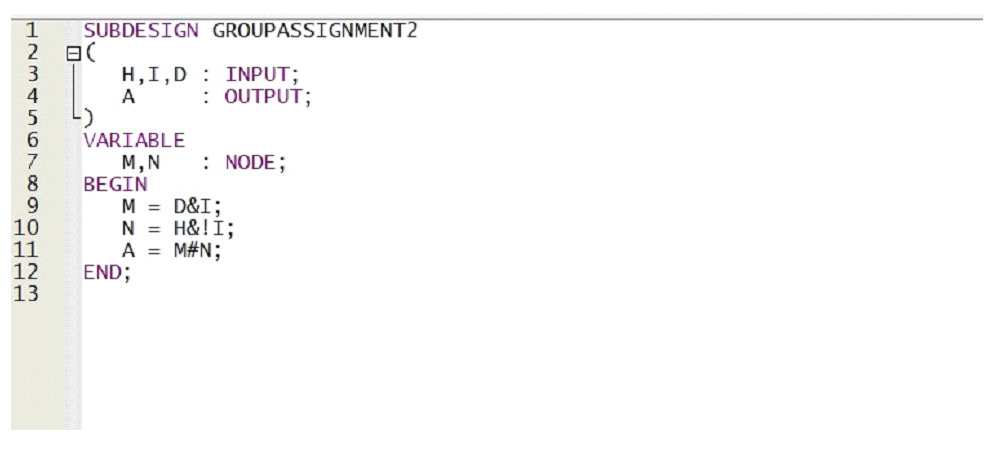
\includegraphics[width=\linewidth]{q2code.png}
    \caption{ The AHDL code for the circuit in question 2}
    \label{fig:q2code}    
\end{figure}
\begin{figure}[H]
    \centering
    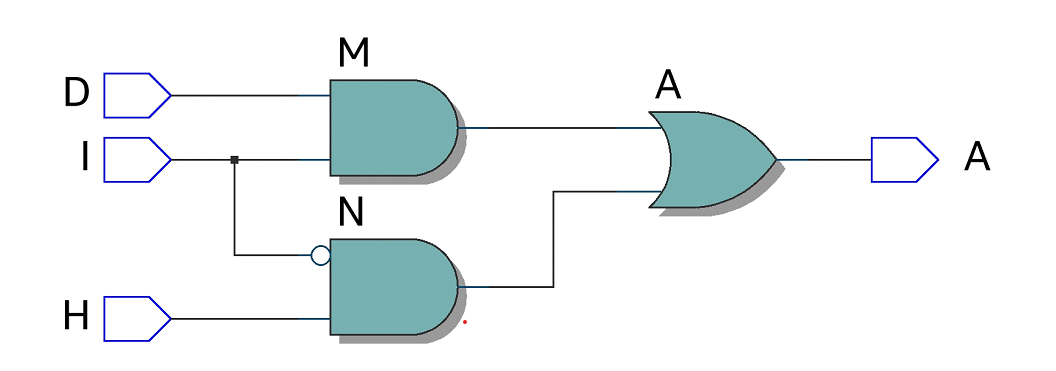
\includegraphics[width=\linewidth]{q2schem.png}
    \caption{ The Quartus generated schematic for the circuit in question 2}
    \label{fig:q2schem}    
\end{figure}
\begin{figure}[H]
    \centering
    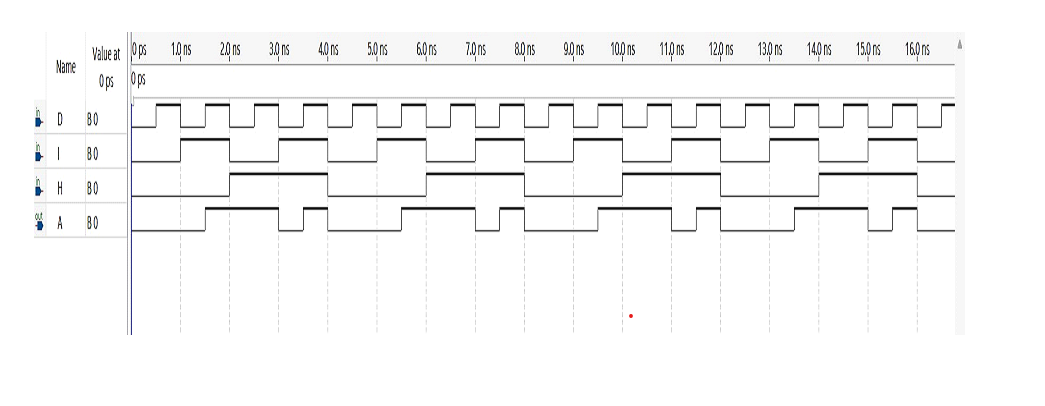
\includegraphics[width=\linewidth]{q2timi.png}
    \caption{   Timing diagram for the circuit in question 2}
    \label{fig:q2timi}    
\end{figure}



\newpage
\section*{Question 3}
The following figure shows four switches that are part of the control circuitry in a
copy machine. The switches are at various points along the path of the copy
paper as the paper passes through the machine. Each switch is normally open,
and as the paper passes over a switch, the switch closes. It is impossible for
switches SW1 and SW4 to be closed at the same time.

\begin{figure}[H]
    \centering
    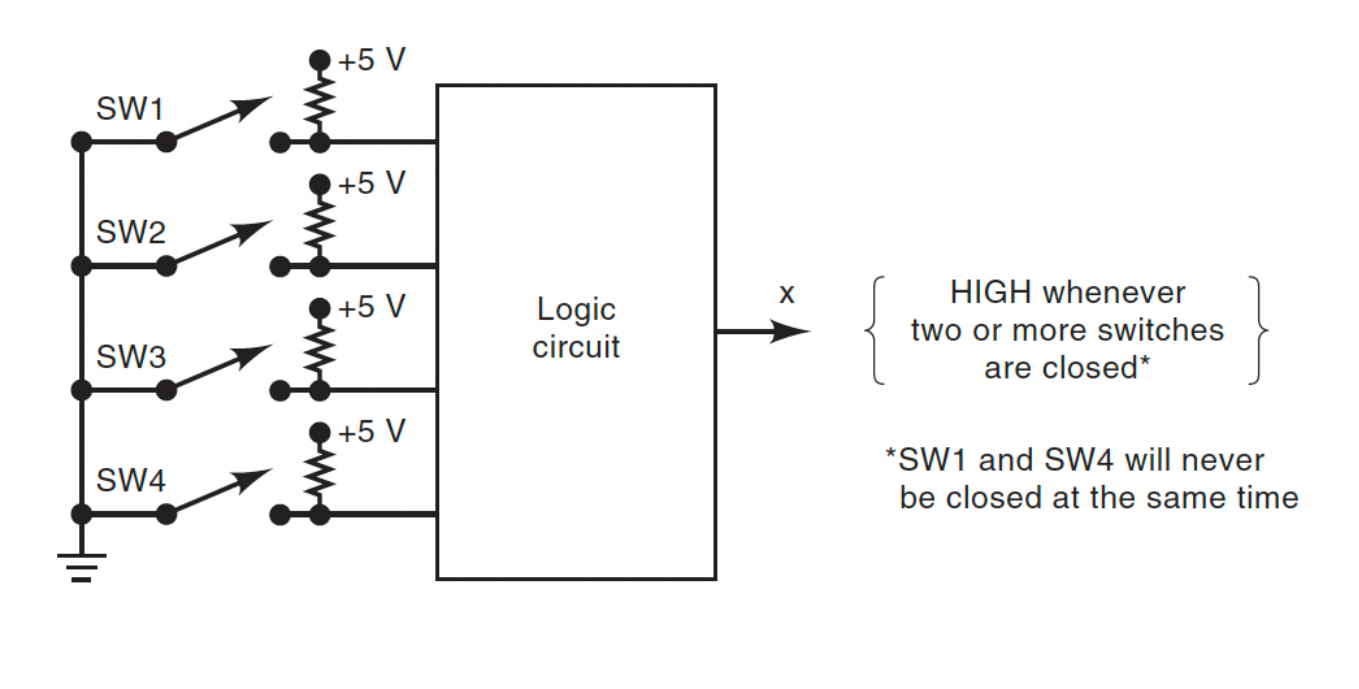
\includegraphics[width=0.6\linewidth]{q3.png}
    \caption{Four switches that are part of the control circuitry in a copy machine}
    \label{fig:q3}
\end{figure}

\subsection*{(a)} \textbf{Design the logic circuit to produce a HIGH output whenever two or more
switches are closed at the same time. Use K mapping and take advantage
of the don`t-care conditions.}

\begin{center}
\begin{tabular}{cccc|c|c}
    SW4 & SW3 & SW2 & SW1 & Y & \\ \hline
    0 & 0 & 0 & 0 & x & \\
    0 & 0 & 0 & 1 & 1 & $\olsi{SW4} \olsi{SW3} \olsi{SW2} SW1$\\
    0 & 0 & 1 & 0 & x & \\
    0 & 0 & 1 & 1 & 1 & $\olsi{SW4} \olsi{SW3} SW2 SW1$\\
    0 & 1 & 0 & 0 & x & \\
    0 & 1 & 0 & 1 & 1 & $\olsi{SW4} SW3 \olsi{SW2} SW1$\\
    0 & 1 & 1 & 0 & x & \\
    0 & 1 & 1 & 1 & 0 & \\
    1 & 0 & 0 & 0 & 1 & $SW4 \olsi{SW3} \olsi{SW2} \olsi{SW1}$\\
    1 & 0 & 0 & 1 & 1 & $SW4 \olsi{SW3} \olsi{SW2} SW1$\\
    1 & 0 & 1 & 0 & 1 & $SW4 \olsi{SW3} SW2 \olsi{SW1}$\\
    1 & 0 & 1 & 1 & 0 & \\
    1 & 1 & 0 & 0 & 1 & $SW4 SW3 \olsi{SW2} \olsi{SW1}$\\
    1 & 1 & 0 & 1 & 0 & \\
    1 & 1 & 1 & 0 & 0 & \\
    1 & 1 & 1 & 1 & 0 & \\

\end{tabular}
\end{center}

\begin{center}
\begin{karnaugh-map}[4][4][1][SW1][SW2][SW3][SW4]
    \manualterms{x,1,x,1,x,1,x,0,1,1,1,0,1,0,0,0}
    \implicant{0}{2}
    \implicant{0}{5}
    \implicant{0}{8}
    \implicantedge{0}{1}{8}{9}
    \implicantcorner
\end{karnaugh-map}
\end{center}

\[Y = \olsi{SW4}\olsi{SW3} + \olsi{SW4}\olsi{SW2}+\olsi{SW2}\olsi{SW1}+\olsi{SW3}\olsi{SW2}+\olsi{SW3}\olsi{SW1}\]

\begin{center}
\begin{circuitikz}
    \draw
    (7,0) node[and port] (s13) {}
    (7,2) node[and port] (s43) {}
    (7,4) node[and port] (s12) {}
    (7,6) node[and port] (s42) {}
    (7,8) node[and port] (s23) {}

    
    (1,2) node[not port, scale = 0.6] (sw1) {}
    (1,4) node[not port, scale = 0.6] (sw2) {}
    (1,6) node[not port, scale = 0.6] (sw3) {}
    (1,8) node[not port, scale = 0.6] (sw4) {}
    
    (11,4) node[or port, number inputs=5] (or) {}

    (s13.out) -- ++(2,0) |- (or.in 5)
    (s43.out) -- ++(1,0) |- (or.in 4)
    (s12.out) -- ++(0,0) |- (or.in 3)
    (s42.out) -- ++(1,0) |- (or.in 2)
    (s23.out) -- ++(2,0) |- (or.in 1)
    
    (or.out) to[short, -o] ++(1,0) node[label=right:$Y$] {}
    (0, 2) node[label=left:SW1] {} to[short,*-] (sw1.in)
    (0, 4) node[label=left:SW2] {} to[short,*-] (sw2.in)
    (0, 6) node[label=left:SW3] {} to[short,*-] (sw3.in)
    (0, 8) node[label=left:SW4] {} to[short,*-] (sw4.in)

    (sw1.out)  to[short,-*] ++(3.5,0)|- (s13.in 1)
    (sw3.out)  to[short,-*] ++(2.8,0)|- (s13.in 2)
    
    (sw4.out)  to[short,-*] ++(2.1,0)|- (s43.in 1)
    (sw3.out)  to[short,-*] ++(1.4,0)|- (s43.in 2)
    
    (sw1.out)  to[short,-*] ++(0.3,0)|- (s12.in 1)
    (sw2.out)  to[short,-*] ++(0.6,0)|- (s12.in 2)
    
    (sw4.out)  to[short,-*] ++(1.2,0)|- (s42.in 1)
    (sw2.out)  to[short,-*] ++(1.8,0)|- (s42.in 2)
    
    (sw1.out)  to[short,-*] ++(2.4,0)|- (s23.in 1)
    (sw2.out)  to[short,-*] ++(3.2,0)|- (s23.in 2)

;\end{circuitikz}
\end{center}

\subsection*{(b)} \textbf{Use Quartus software to implement the circuit in (a). Show the code, RTL
viewer schematic, and timing diagram of the circuit performance}

\begin{figure}[H]
    \centering
    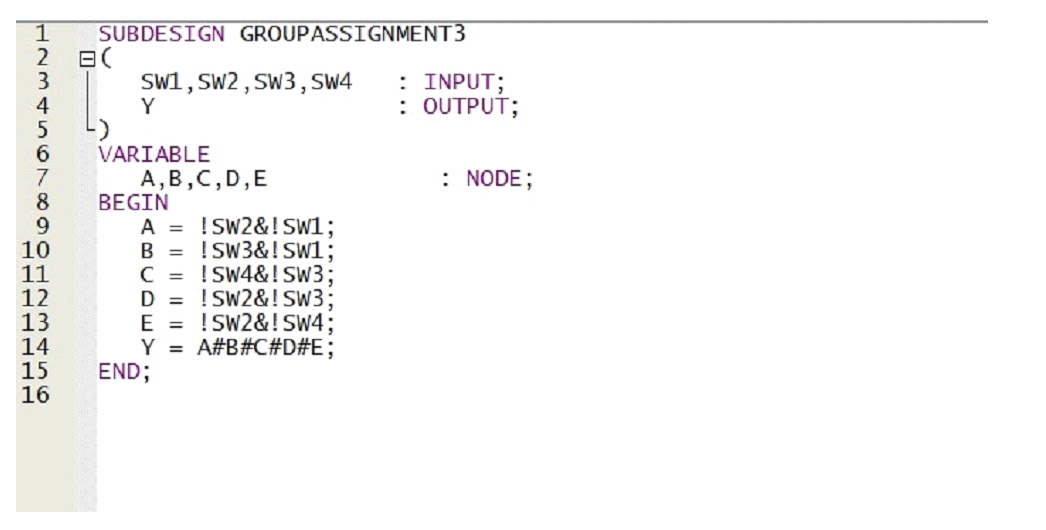
\includegraphics[width=\linewidth]{q3code.png}
    \caption{ The AHDL code for the circuit in question 3}
    \label{fig:q3code}    
\end{figure}
\begin{figure}[H]
    \centering
    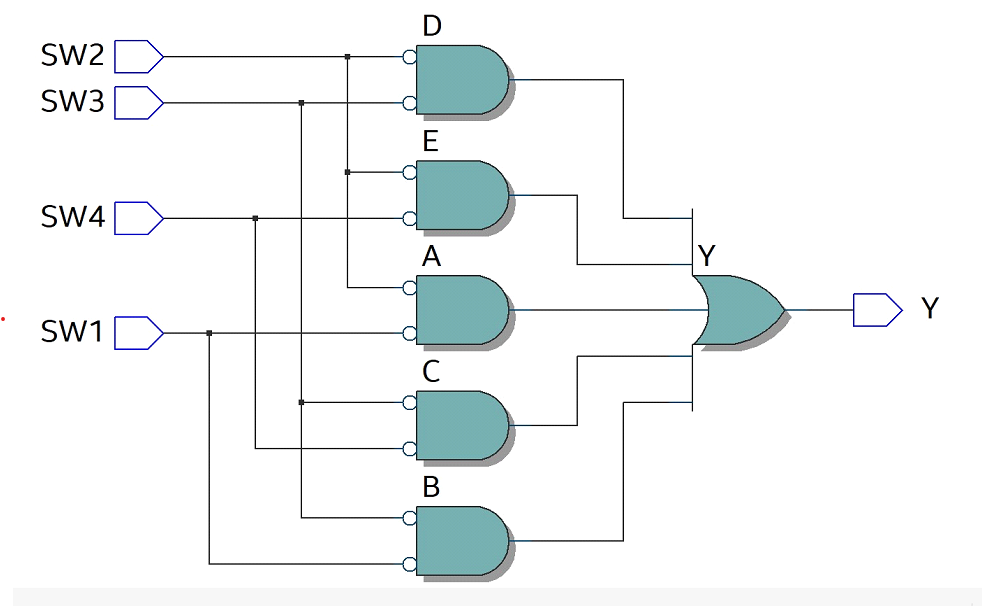
\includegraphics[width=\linewidth]{q3schem.png}
    \caption{ The Quartus generated schematic for the circuit in question 3}
    \label{fig:q3schem}    
\end{figure}
\begin{figure}[H]
    \centering
    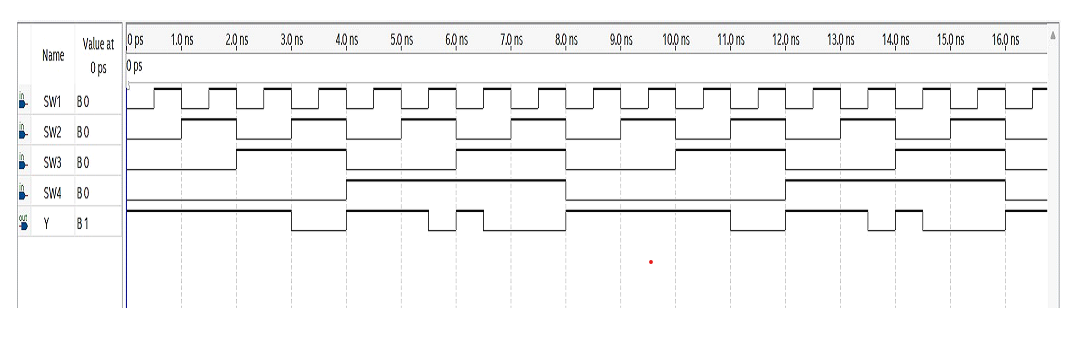
\includegraphics[width=\linewidth]{q3timi.png}
    \caption{  Timing diagram for the circuit in question 3}
    \label{fig:q3timi}    
\end{figure}


\end{document}